\subsection{Performance Requirements}
\begin{itemize}
\textbf{Response Time}: The system must allow users to log in and edit their profiles without  minimum wait time. The response time must be the must not vary for the same function executed numerous times.\\	\\

\textbf{Scalability}: The system must perform adequately no matter how many users are using the system concurrently.
	
\end{itemize}
\subsection{Design Constraints}
\begin{enumerate}
	
\end{enumerate}
\subsection{Software System Attributes}
{ 
    \begin{flushleft}
    \par\textbf{Accuracy: }Users' information must be correct and must record any changes to their profiles accurately.\newline
    
    \par\textbf{Availability: }Users' profile must always be available to the users whenever the need to log in or edit their profiles.\newline
}


\subsection{Class diagram}
 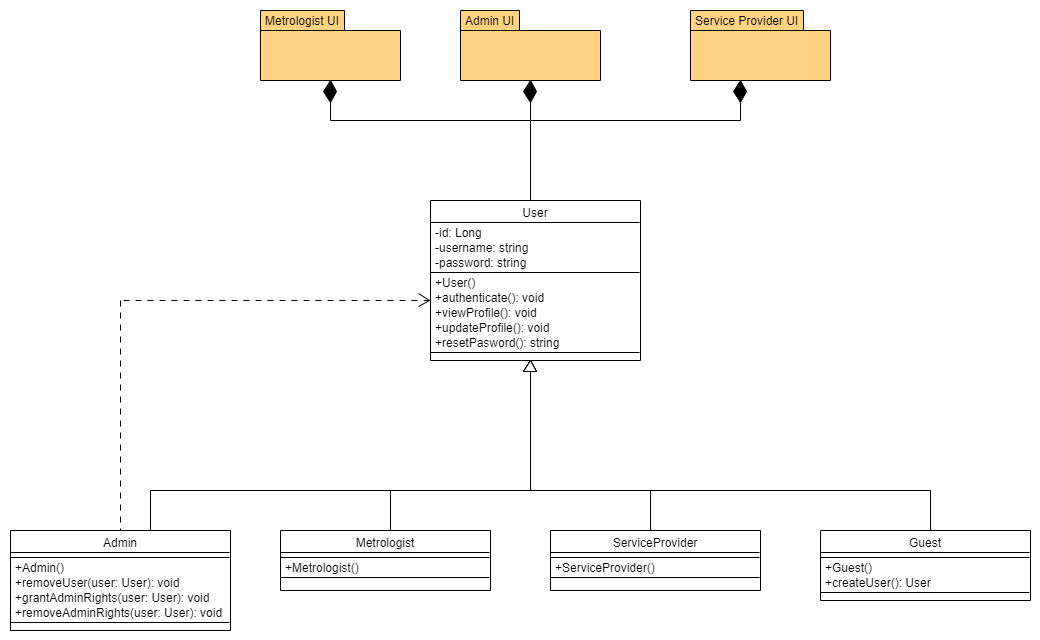
\includegraphics[width=12cm,height=26cm,keepaspectratio]{users_unit/Images/users_class_diagram.png}
	\begin{center}
	    \small{Figure 6: Class diagram for Users}
    \end{center}
	\paragraph{Design Patterns Used} \\ \\\\
	
	The Template method design pattern was used for the Users sub-system. The different users of the benchmarking system, Hub admins, metrologists and service providers, have similar functions. They all have functionality to change profile information and to reset passwords. Template method allows code reuse for these shared functions while allowing the other user functionality to differ.
	
		
\subsection{Activity diagram}
    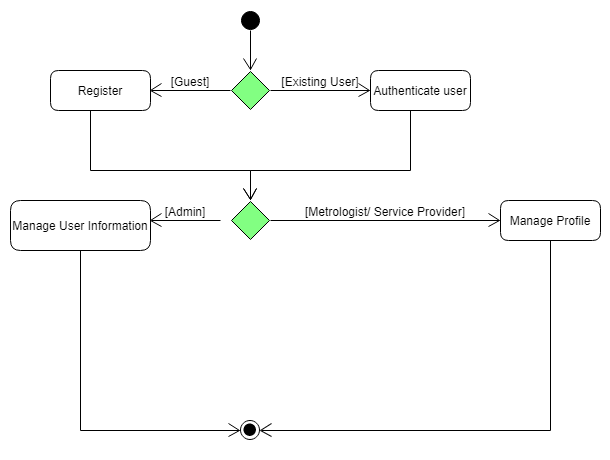
\includegraphics[width=12cm,height=26cm,keepaspectratio]{users_unit/Images/users_activity_diagram.png}
	\begin{center}
	    \small{Figure 7: Activity diagram for Users}
    \end{center}


\subsection{Sequence diagram}
    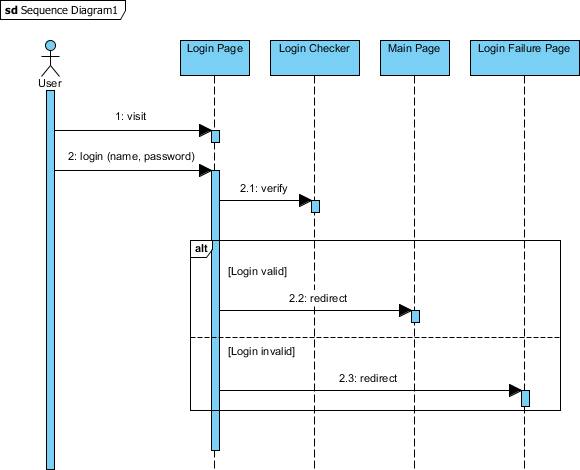
\includegraphics[width=12cm,height=26cm,keepaspectratio]{users_unit/Images/users_sequence_diagram.png}
	\begin{center}
	    \small{Figure 8: Sequence diagram for Users }
    \end{center}

\subsection{State diagram}
    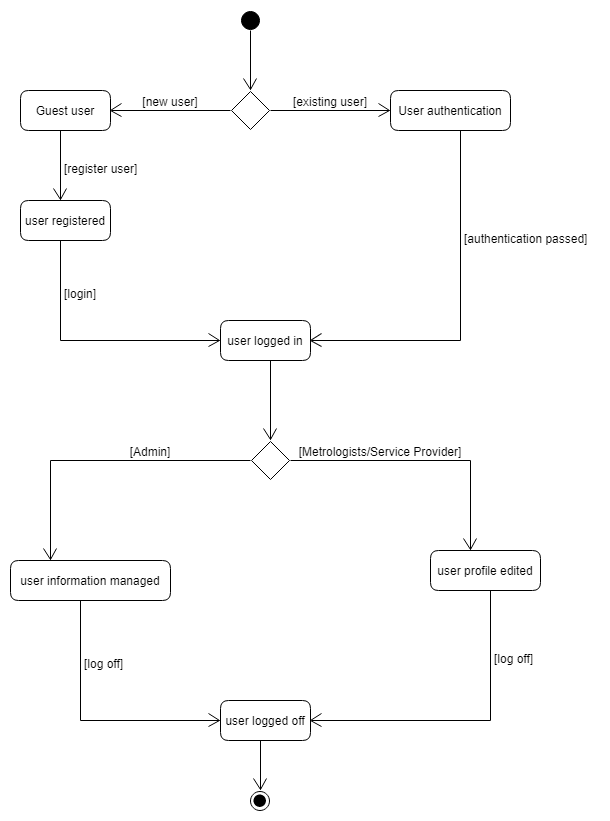
\includegraphics[width=12cm,height=26cm,keepaspectratio]{users_unit/Images/users_state_diagram.png}
	\begin{center}
	    \small{Figure 9: State diagram for Users}
    \end{center}




\subsection{Use Case diagram}
   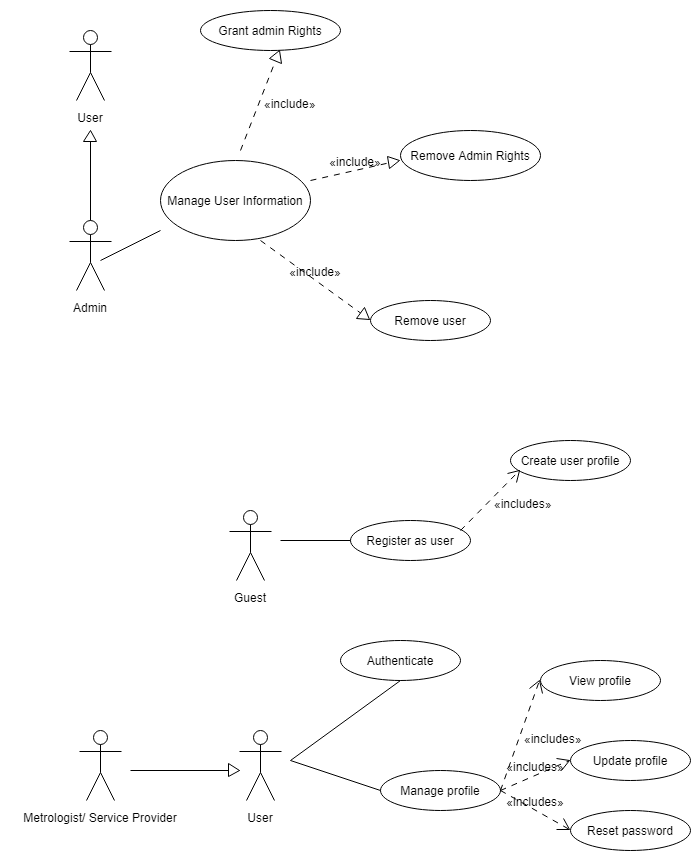
\includegraphics[width=12cm,height=26cm,keepaspectratio]{users_unit/Images/users_use_case_diagram.png}
    \begin{center}
    	\small{Figure 10: Use case diagram for Users}
    \end{center}